\section{Impact Across User Groups}%
\label{sec:usage}

The Semantic Web Language Server (SWLS) was designed to address the diverse needs of practitioners engaging with semantic web technologies. This section reflects on the challenges faced by the user groups introduced in Section \ref{sec:introduction} and demonstrates how the SWLS alleviates these through its features. A live demo of SWLS, available at \url{swls.ajuvercr.be}, showcases its capabilities across four editor interfaces:

\begin{enumerate}
  \item Turtle Editor for data management
  \item OWL Editor for ontology creation
  \item SHACL Editor for shape constraints
  \item SPARQL Editor for crafting queries
\end{enumerate}

While all editors, except for the SPARQL editor, are functionally the same, 
the visual seperation improves the realism of the tasks at hand.
Below, we discuss how SWLS benefits each user group and validate its utility in practice.

We first go over the key ways the SWLS might help users, then we will apply these ways to the different user groups defined in Section \ref{sec:introduction}, 
and how those users groups are theorectially assisted by the SWLS.

\subsection{Key Improvements by SWLS}

The SWLS significantly enhances development efficiency by incorporating robust autocompletion features, shown in Figure \ref{class_completion} and Figure \ref{property_completion}.
These features streamline the creation of semantic documents, enabling users to work faster and with fewer errors. 
Whether defining ontologies, creating SHACL shapes, or writing SPARQL queries, the ability to suggest appropriate classes and properties reduces repetitive tasks and minimizes the cognitive load on users, allowing them to focus on the substance of their work.
Autocompletions also helps user explore the current domain by providing context-aware suggestions.

SWLS also aims to improve comprehension by offering real-time feedback on semantic data.
The hover feature (shown in Figure \ref{hover}), which displays detailed information such as associated classes, allows users to quickly grasp the structure and relationships within a document. 
This instant access to contextual information reduces the need for external references and improves overall productivity.

Finally, SWLS aims to increase user confidence in both syntax and semantics
Syntax validation ensures that documents adhere to the expected standards, catching common mistakes as they occur. This feature is shown in Figure \ref{undefined_prefix}.
For semantic validation, the server highlights SHACL violations, helping users align their documents with structural and logical constraints, shown in Figure \ref{shacl_validation}. 
These validation features not only enhance document quality but also provide educational feedback, aiding users in their journey to master semantic web technologies.

\begin{figure}[h!tb]
    \centering
    % code1
    \begin{subfigure}{0.48\textwidth}
      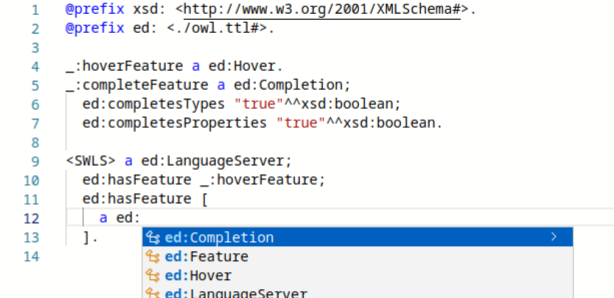
\includegraphics[width=\textwidth]{./images/class_complete.png}
      \caption{SWLS completes a class when the user want to specify the class}
      \label{class_completion}
    \end{subfigure}
    \hfill
    % code 2
    \begin{subfigure}{0.48\textwidth}
      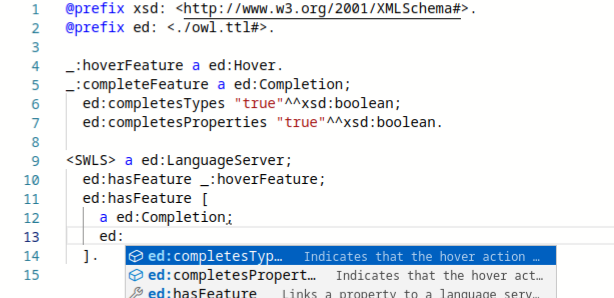
\includegraphics[width=\textwidth]{./images/property_complete.png}
      \caption{SWLS completes properties, first the properties with the correct domain}
      \label{property_completion}
    \end{subfigure}
    \hfill
    % undefined prefix
    \todo{Actually add those screenshots}
    \begin{subfigure}{0.48\textwidth}
      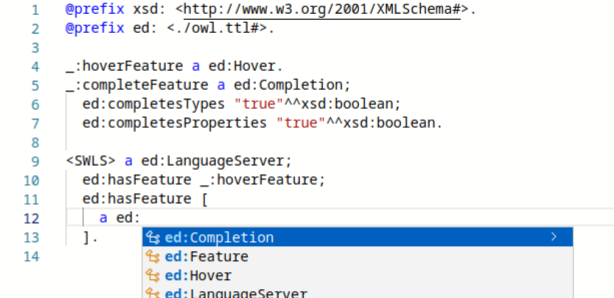
\includegraphics[width=\textwidth]{./images/class_complete.png}
      \caption{SWLS notifies the user of undefined prefixes}
      \label{undefined_prefix}
    \end{subfigure}
    \hfill
    % shacl validation
    \begin{subfigure}{0.48\textwidth}
      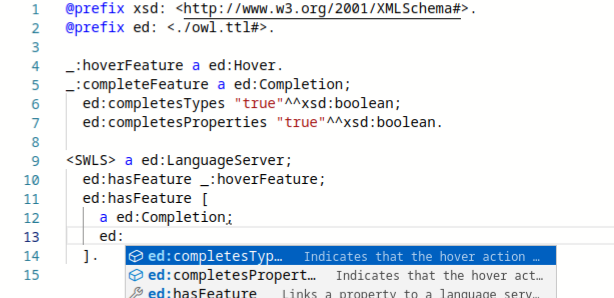
\includegraphics[width=\textwidth]{./images/property_complete.png}
      \caption{SWLS notifies the user of SHACL violations}
      \label{shacl_validation}
    \end{subfigure}
    \hfill
    % shacl validation
    \begin{subfigure}{0.48\textwidth}
      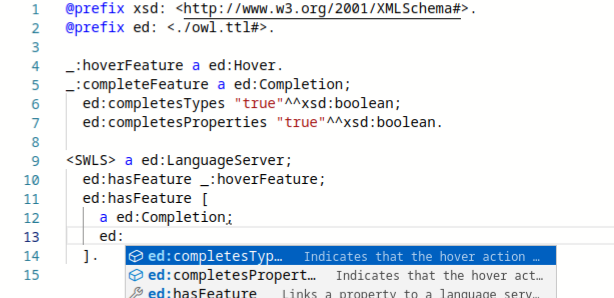
\includegraphics[width=\textwidth]{./images/property_complete.png}
      \caption{SWLS notifies the user of SHACL violations}
      \label{hover}
    \end{subfigure}
    \hfill
    \caption{
      Demo application that shows the usage of SWLS.
      It helps the user by providing autocompletion on classes and properties, taking into account the domain of the properties.
      SWLS also notifies the user of issues like undefined prefixes and SHACL violations.
    }\label{lst:Demo}
\end{figure}

\todo{Add screenshots}

\subsection{User groups}

\paragraph{Semantic power users,} who frequently interact with semantic web technologies, rely on their deep understanding of common properties and domain-specific knowledge to navigate tasks efficiently.
SWLS enhances their workflows by providing robust autocompletion features that streamline document creation and reduce repetitive tasks.
For these users, SWLS also offers a valuable tool for exploring new domains through property suggestions, enabling them to adapt to unfamiliar contexts more easily. 
Additionally, the language server supports quality assurance by helping power users identify common pitfalls such as punning or poorly structured ontologies, ensuring their semantic documents are both accurate and high quality.

\paragraph{For newcomers to the semantic web,} engaging with these technologies can be daunting due to challenges with syntax, semantics, and validation. 
SWLS addresses these pain points by providing immediate feedback on syntax errors, which helps users learn the correct structure and prevents frustration.
The autocompletion feature offers guided support by suggesting relevant properties, allowing users to build confidence in creating semantic documents.
Moreover, validation tools play an educational role: newcomers can intentionally trigger SHACL validation errors to understand what constitutes a faulty document,
turning mistakes into valuable learning opportunities.

\paragraph{Domain experts,} a subset of power users, focus on their specialized fields of knowledge. 
While they share many of the same benefits as general power users, they primarily use SWLS to refine ontologies and ensure alignment with domain-specific standards. 
The autocompletion and hover documentation features help domain experts ensure precision and consistency, facilitating the creation of detailed and accurate semantic models tailored to their expertise.

\paragraph{Data engineers,} on the other hand, primarily work with SPARQL queries to extract meaningful insights from semantic data. 
For these users, SWLS provides critical support by offering autocompletion for classes and properties, as well as syntax validation to prevent errors during query formulation. 
These features significantly enhance productivity by reducing the time spent debugging queries and ensuring accurate results. 
By streamlining the querying process, SWLS enables data engineers to focus on deriving insights rather than resolving technical challenges.

% \subsection*{Semantic Power Users}
% Power users, who frequently interact with RDF datasets, ontologies, and queries, benefit from SWLS’s seamless diagnostics, real-time autocompletion, and syntax highlighting. 
% These features ensure a smoother workflow and fewer errors in their day-to-day tasks.
% For example, in the demo’s Turtle editors, 
%   the power user uses autocompletion to improve development efficiency while writing sample data and OWL definitions, this is shown in Figure \ref{class_completion} and \ref{property_completion}.
% The suggested properties first show the properties that align with the domain of the property definition.
% It is not incorrect to use properties when the domain does not align, so these properties are shown as well.
% If the domain property aligns, the completion kind is \texttt{FIELD} otherwise just \texttt{PROPERTY}.
%
% - Semantic power user -> often, interacts with semantic web technologies
% - user knows common properties, effienct use of autocomplete (knows what to expect)
% - user is challenged by new domains (just like newcomer can use autocompletion to explore doamins)
% - user knows common pitfals in domain and uses SWLS to more easily verify the quality of the semantic web document (punning, ...)
%
%
% \subsection*{Newcomers to the Semantic Web}
% New users often struggle with understanding semantic web standards and crafting accurate queries.
% The demo illustrates how SWLS aims to lower the barrier to entry by providing autocompletions and hover-based explanations for properties and classes. 
% These features aims to help users to explore ontologies dynamically, fostering learning and confidence, an examples is shown in Figure \ref{hover}.
% SWLS also validating the data, aiming to increase confidence in the users data. 
% An undefined prefix error is shown in Figure \ref{undefined_prefix} and a SHACL validation error is shown in Figure \ref{shacl_validation}.
%
% - Dables maybe for the first time in semantic web technologies, which is quite confusing
% - Wants to get to know the technologies, bumping into the syntax, semantics and validation.
% - SWLS helps these users by giving instant feedback on syntax, helps find the most fitting properties, 
%   but also help the confidence of the user by trigging SHACL validation errors (which the user might even do on purpose to know how to make a document faulty)
%
% \subsection*{Domain Experts}
% For domain experts who typically rely on tools like Protégé for ontology development, SWLS offers a streamlined alternative. 
% In the Demo, the domain expert can write the ontology in the Ontology editor and get a feeling of how users would use that ontology by creating sample data and sample queries.
% This approach is particularly useful for smaller or ad-hoc projects.
%
%
% \subsection*{Data Engineers}
% Data engineers rely on tools to simplify complex SPARQL query creation and optimize ontology integration. 
% The SPARQL editor in the demo exemplifies SWLS’s ability to provide meaningful assistance. 
% Context-aware autocompletions, hover-based information, and diagnostics for undefined properties enable engineers to craft queries with greater precision.
%

\subsection{Continuous Development}

SWLS is not static software: its extensible design ensures that new features and improvements can be easily incorporated. 
The current implementation provides a robust foundation for further exploration of user needs and iterative enhancement.

For examples,
users that interact with ComponentsJS (CJS) configurations have a difficult time\cite{CJS}, often checking the correctness of their configuration at runtime.
Normal JSON-LD editors have difficulties to handle CJS configuration because of the used Linked Software Dependencies\cite{CJS2}, that should be resolved to the local \texttt{node\_modules} folders.
By adding two things to SWLS, CJS users can use the same powerful IDE support as other semantic web developers.
\begin{enumerate}
  \item Add a new way to resolve JSON-LD contexts, by looking for the write configuration files in the \texttt{node\_modules}.
  \item Derive properties from CJS component definitions
  \item Validate configuration by using the checking if all parameters are defined and have the correct range.

\end{enumerate}


\subsection{IDE integration}

\subsubsection{Monaco online demo}
\subsubsection{Visual Studio Code}
\subsubsection{Neo Vim}

% How does ecs scale for new features?
% How can the LSP be integrated in the setup for the end user.
% Maybe some performance metrics? Cost to run it
% Running in the browser, this tool might be integrated in new/existing sparql query tools

